\documentclass[10pt,a4paper]{article}
\usepackage[utf8]{inputenc}
\usepackage[T1]{fontenc}
\usepackage[spanish,es-nodecimaldot]{babel}
\usepackage{lmodern}
\usepackage{microtype}
\usepackage{geometry}
\geometry{margin=2.2cm}
\usepackage{amsmath,amssymb,booktabs,graphicx,hyperref,xcolor}
\usepackage[backend=biber,style=numeric,sorting=none,maxbibnames=8]{biblatex}
\addbibresource{referencias.bib}
\hypersetup{colorlinks=true,linkcolor=blue!45!black,citecolor=blue!45!black,urlcolor=blue!45!black}
\setlength{\parindent}{0pt}
\setlength{\parskip}{0.45em}

\title{Detección no supervisada de anomalías en radiografías de tórax\\mediante AE, VAE y GAN}
\author{Trabajo Fin de Máster\\Máster Universitario en Sistemas Inteligentes}
\date{Curso 2025--2026}

\begin{document}
\maketitle

\begin{abstract}
La escasez de anotaciones clínicas exhaustivas limita el entrenamiento de
detectores supervisados capaces de reconocer patologías diversas. Este trabajo
estudia si un modelo entrenado exclusivamente con radiografías normales puede
asignar una puntuación alta a imágenes no normales. Se comparan, bajo un mismo
protocolo, un autoencoder convolucional (AE), un autoencoder variacional (VAE) y
GANomaly, una arquitectura adversarial. Se emplea Chest-RSNA, la partición de
radiografías del benchmark BMAD: 8.000 imágenes normales para entrenamiento,
1.490 para validación y 17.194 para prueba. En tres semillas, GANomaly obtiene
AUROC $0{,}5636\pm0{,}0150$, por encima de AE ($0{,}4566\pm0{,}0163$) y VAE
($0{,}4506\pm0{,}0016$). Un control de gradiente alcanza 0,5981. Como referencia
práctica se añade un único clasificador convolucional supervisado, que logra
$0{,}8538\pm0{,}0070$ sin consultar el test durante el desarrollo. El contraste
muestra que las etiquetas aportan una señal que los métodos de reconstrucción
no captan. La contribución es una comparación reproducible, no un diagnóstico.
\end{abstract}

\section{Contextualización y motivación}

\subsection{Problema}

La imagen médica es una fuente central de información diagnóstica, pero un
algoritmo convencional necesita ejemplos representativos y correctamente
etiquetados de cada entidad que deberá reconocer. En radiología, obtener esas
etiquetas exige tiempo experto, los hallazgos pueden ser sutiles, existe
variabilidad entre observadores y la distribución de patologías es muy
desigual. Además, un clasificador cerrado aprende las categorías disponibles y
puede responder con excesiva confianza ante un patrón no representado. Estas
condiciones motivan la detección de anomalías: modelar la normalidad y señalar
desviaciones sin exigir ejemplos de todas las enfermedades posibles
\cite{pang2021review,ruff2021unifying}.

La formulación de una clase es especialmente natural cuando abundan muestras
sanas y las anomalías son heterogéneas. Sea $x$ una radiografía y $f_\theta$ un
modelo ajustado con el conjunto normal $\mathcal{D}_{N}$. Se busca una función
$s(x)$ tal que
\[
  s(x_N) < s(x_A), \qquad x_N\sim p_N,\quad x_A\not\sim p_N,
\]
sin utilizar $x_A$ para optimizar $\theta$. El resultado no es un diagnóstico,
sino una puntuación de incompatibilidad con la distribución aprendida.

\subsection{Por qué reconstrucción generativa}

Un autoencoder comprime la entrada en una representación latente y aprende a
reconstruirla \cite{hinton2006reducing}. Si solo observa imágenes normales, se
espera que reconstruya peor una alteración y que el residuo sirva como señal de
anomalía. La hipótesis es atractiva, pero no está garantizada: una red con mucha
capacidad puede copiar también una entrada anómala; el error puede estar
dominado por contraste, bordes o adquisición, y una reconstrucción visualmente
nítida no implica mejor discriminación \cite{baur2021autoencoders}.

El VAE introduce una representación probabilística regularizada mediante la
divergencia de Kullback--Leibler \cite{kingma2014vae}. Esto puede producir un
espacio latente más continuo, aunque también reconstrucciones suavizadas. Las
GAN enfrentan generador y discriminador \cite{goodfellow2014gan}; aplicaciones
como AnoGAN y GANomaly trasladan ese aprendizaje adversarial a detección de
anomalías \cite{schlegl2017anogan,akcay2019ganomaly}. La literatura médica
incluye autoencoders adversariales, VAE en cascada y autoencoders enmascarados
\cite{zhang2022improved,guo2021cvad,georgescu2023masked}. No obstante, las
diferencias de datasets, preprocesado y métricas dificultan saber qué parte de
la mejora procede realmente del modelo.

\subsection{Pregunta de investigación y alcance}

La pregunta principal es: \emph{¿qué familia, AE, VAE o GANomaly, separa mejor
radiografías normales y no normales cuando todas se entrenan solo con normales
y se evalúan bajo idénticas condiciones?}

El estudio usa radiografías frontales del benchmark Chest-RSNA de BMAD
\cite{bao2024bmad,shih2019rsna}. ``Anómala'' significa \emph{no normal según la
taxonomía RSNA/BMAD}; no significa cualquier patología torácica ni confirma
neumonía. La salida podría servir como señal de priorización o control de
calidad en investigación, pero el sistema no está calibrado prospectivamente,
no ha sido validado externamente y no debe utilizarse para decisiones clínicas.

\subsection{Aportaciones}

Las aportaciones concretas son: (i) selección y auditoría reproducible de un
conjunto público adecuado; (ii) implementaciones comparables de AE, VAE y
GANomaly; (iii) separación estricta entre ajuste, selección de umbral y prueba;
(iv) evaluación con métricas robustas al desequilibrio y análisis de coste; y
(v) una referencia supervisada mínima que cuantifica el valor de disponer de
etiquetas; y (vi) publicación del código y de la configuración, sin redistribuir
imágenes médicas.


\section{Objetivos}

\subsection{Objetivo general}

Diseñar, implementar y evaluar un sistema reproducible de detección no
supervisada de anomalías en radiografías de tórax, comparando un AE, un VAE y
una alternativa adversarial GAN bajo un protocolo común.

\subsection{Objetivos específicos y criterios de logro}

\begin{enumerate}
  \item \textbf{Revisar el estado del arte} de detección de anomalías basada en
  reconstrucción, identificando supuestos, funciones de pérdida, puntuaciones y
  riesgos. Se considera cumplido al justificar las tres familias y el protocolo
  a partir de bibliografía primaria.

  \item \textbf{Obtener y preparar un dataset médico adecuado.} Debe contener
  radiografías normales y anómalas, entrenamiento normal, validación y prueba.
  Se verifica mediante conteos, lectura de imágenes, dimensiones y control de
  duplicados exactos entre particiones.

  \item \textbf{Implementar tres modelos comparables}: AE convolucional, VAE y
  GANomaly. Deben compartir resolución, dimensión latente, optimizador,
  presupuesto de épocas y semillas, y producir una puntuación por imagen.

  \item \textbf{Definir una evaluación sin fuga de información.} Los pesos se
  ajustan solo con entrenamiento normal; el checkpoint se selecciona con
  validación normal; las etiquetas completas de validación fijan el umbral; el
  test se consulta una vez con el método congelado.

  \item \textbf{Comparar efectividad y coste}. La métrica principal es AUROC de
  test; se reportan AUPRC, exactitud balanceada, sensibilidad, especificidad,
  F1, número de parámetros y tiempo. La afirmación de superioridad requiere la
  media de tres semillas y dispersión, no una ejecución aislada.

  \item \textbf{Analizar limitaciones y reproducibilidad}. Se documentan
  desequilibrio, sesgos de adquisición, pérdida por redimensionado, significado
  limitado de la etiqueta y ausencia de validación clínica externa.

  \item \textbf{Establecer una referencia supervisada simple}. Un único
  clasificador debe reutilizar el codificador existente, mantener el test
  intacto y mostrar si las etiquetas permiten una separación más útil.
\end{enumerate}

Quedan fuera del alcance mínimo la localización de lesiones, la clasificación
por patología, el uso asistencial y la comparación exhaustiva con métodos
preentrenados modernos. Son extensiones válidas, pero diluirían la pregunta
central y el presupuesto de un TFM individual de 18 ECTS.


\section{Fundamentos y estado del arte}

\paragraph{AE.} Minimiza el error de reconstrucción
$\mathcal{L}_{AE}=\lVert x-g_\theta(f_\phi(x))\rVert_1$. Su ventaja es la
simplicidad; su debilidad es que el cuello de botella no impone una distribución
latente y puede generalizar la reconstrucción fuera de la normalidad.

\paragraph{VAE.} Aproxima $q_\phi(z\mid x)$ mediante una normal parametrizada y
optimiza
\[
\mathcal{L}_{VAE}=\lVert x-\hat{x}\rVert_1+
\beta D_{KL}\!\left(q_\phi(z\mid x)\,\|\,\mathcal{N}(0,I)\right).
\]
El truco de reparametrización permite derivar a través del muestreo
\cite{kingma2014vae}. Estudios recientes comparan variantes convolucionales y
transformers y confirman que la arquitectura y $\beta$ condicionan el resultado
\cite{nguyen2024vae}.

\paragraph{GANomaly.} Frente a la optimización iterativa de AnoGAN, GANomaly
aprende dos codificadores y un decodificador. Su generador produce
$z=E_1(x)$, $\hat{x}=G(z)$ y $\hat{z}=E_2(\hat{x})$. Combina pérdida contextual,
latente y adversarial; durante inferencia, $\lVert z-\hat{z}\rVert_1$ actúa como
puntuación \cite{akcay2019ganomaly}. La comparación es relevante porque el
entrenamiento adversarial puede mejorar representaciones, pero añade
inestabilidad y coste.

Los benchmarks industriales como MVTec AD impulsaron protocolos comunes
\cite{bergmann2019mvtec}. En medicina, BMAD extiende esa idea a seis conjuntos
de cinco dominios y quince algoritmos \cite{bao2024bmad}. Este trabajo no busca
reproducir todo el leaderboard: aísla las tres familias solicitadas en la
propuesta y controla las variables experimentales.


\section{Datos y metodología}

\subsection{Chest-RSNA}

BMAD reorganiza las 26.684 radiografías del desafío RSNA en el formato de
detección de anomalías. Entrenamiento contiene 8.000 normales; validación, 70
normales y 1.420 anómalas; test, 781 normales y 16.413 anómalas. La auditoría
local confirmó los conteos, el formato PNG, escala de grises y resolución
1024$\times$1024. Una inspección completa con hash está disponible como opción
reproducible. El fuerte desequilibrio hace inadecuada la exactitud simple.

Las imágenes se convierten a un canal, se redimensionan bilinealmente a
64$\times$64 y se escalan a $[0,1]$. Esta resolución reduce el coste para CPU y
permite una comparación controlada, pero puede borrar hallazgos pequeños; por
ello se declara como limitación y una repetición a 128$\times$128 constituye la
ablación prioritaria, no una conclusión asumida.

\subsection{Diseño experimental}

Los modelos comparten dimensión latente 64, Adam con tasa $2\cdot10^{-4}$,
lotes de 64 y 20 épocas. Para GANomaly se usan pesos 1, 50 y 1 en las pérdidas
adversarial, contextual y latente. Para VAE se fija $\beta=10^{-4}$, evitando que
la regularización eclipse prematuramente la reconstrucción. Se ejecutan semillas
13, 42 y 73.

AE puntúa mediante MAE por imagen; VAE suma MAE y KL ponderada; GANomaly usa la
distancia latente. Como las escalas no son comparables directamente, se comparan
rankings (AUROC/AUPRC) y cada modelo obtiene su umbral exclusivamente en
validación. Se maximiza exactitud balanceada y, ante empate, se favorece
especificidad. El umbral se aplica sin cambios a test.

La métrica principal es AUROC. AUPRC refleja el rendimiento bajo prevalencia
desigual, aunque debe interpretarse respecto a la alta proporción anómala del
test. La exactitud balanceada evita que una clase numerosa domine; sensibilidad
y especificidad muestran el compromiso clínicamente relevante. Se reportan
media y desviación de las tres semillas, parámetros y tiempo.

La referencia supervisada reutiliza el mismo codificador y sustituye el
decodificador por una salida binaria. De las 1.420 anomalías de validación se
reservan, junto con igual número de normales de entrenamiento, 1.136 imágenes
por clase para ajuste y 284 por clase para validación. La división es
determinista para cada semilla y el test oficial permanece intacto. Se optimiza
entropía cruzada binaria y se elige el checkpoint por AUROC de validación.

\subsection{Reproducibilidad}

El repositorio contiene rutas configurables, semillas deterministas, guardado
de checkpoints, puntuaciones CSV y configuración JSON. Las imágenes y pesos se
excluyen de Git. El informe distingue mediante el
campo \texttt{scientific\_run} una ejecución completa de una prueba limitada,
impidiendo que resultados de humo entren por error en la tabla final.

Como control no neuronal se calcularon nueve estadísticas predefinidas de
intensidad y textura. Cada una se convirtió en distancia absoluta tipificada
respecto al entrenamiento normal. La selección del control y su umbral usaron
solo validación, igual que los modelos.


\section{Resultados y análisis}

\subsection{Verificación y campaña final}

La auditoría encuentra 8.000/1.490/17.194 imágenes en
entrenamiento/validación/test, coincidiendo con BMAD. Una muestra estratificada
de 308 ficheros se abrió correctamente y todos fueron PNG monocromos de
1024$\times$1024. Una ejecución de humo comprobó carga de datos, salida de los
cuatro modelos, métricas y selección del umbral.

La campaña final ejecutó los tres modelos generativos y la referencia
supervisada durante 20 épocas con semillas 13, 42 y 73, usando el test completo.
La tabla presenta media y desviación estándar entre semillas.

\begin{center}
\small
\begin{tabular}{lrrrr}
\toprule
Modelo & Parámetros & AUROC & AUPRC & Bal. acc. \\
\midrule
AE       & 609.857 & 0,4566$\pm$0,0163 & 0,9533 & 0,5105 \\
VAE      & 740.993 & 0,4506$\pm$0,0016 & 0,9526 & 0,5064 \\
GANomaly & 959.586 & 0,5636$\pm$0,0150 & 0,9655 & 0,5484 \\
Clasificador & 175.025 & \textbf{0,8538$\pm$0,0070} & \textbf{0,9913} & \textbf{0,7717} \\
\bottomrule
\end{tabular}
\end{center}

La prevalencia anómala de test es 95,46\%; por eso AUPRC ronda 0,95 incluso en
AE y VAE. Sus AUROC son inferiores a 0,5 en las seis ejecuciones: las anómalas
presentan una mediana de error ligeramente menor que las normales. Reconstruir
bien normalidad no produce aquí una puntuación discriminativa. GANomaly supera
AE y VAE en cada semilla y es el único modelo con separación en la dirección
esperada, pero su exactitud balanceada media queda en 0,55.

La referencia supervisada obtiene AUROC $0{,}8538\pm0{,}0070$ y exactitud
balanceada $0{,}7717\pm0{,}0136$. Las tres ejecuciones alcanzan 0,8459, 0,8565
y 0,8590, por lo que la mejora no depende de una semilla aislada. La comparación
no atribuye superioridad algorítmica directa: el clasificador recibe anomalías
etiquetadas durante el ajuste y los detectores de una clase no.

\subsection{Controles y análisis de errores}

El control de gradiente medio, seleccionado en validación, obtiene AUROC 0,5981
y exactitud balanceada 0,5894. La diferencia centro--borde alcanza 0,5848 y el
control multivariante diagonal 0,5754. Los tres igualan o superan el GANomaly
medio. Por tanto, la hipótesis se acepta solo parcialmente: GANomaly mejora de
forma consistente el AE, pero no demuestra una representación superior a
señales estadísticas simples.

La inspección del GANomaly con mayor AUROC muestra entre los falsos positivos
encuadres pediátricos, rotaciones, marcadores, proyecciones portátiles y cambios
de contraste. Los falsos negativos conservan con frecuencia un encuadre adulto
estandarizado pese a estar etiquetados como no normales. Esta evidencia visual,
junto al control de gradiente, sugiere que parte de la señal procede del proceso
de adquisición y no necesariamente de la patología. No se interpretan las
imágenes clínicamente.

\begin{figure}[ht]
  \centering
  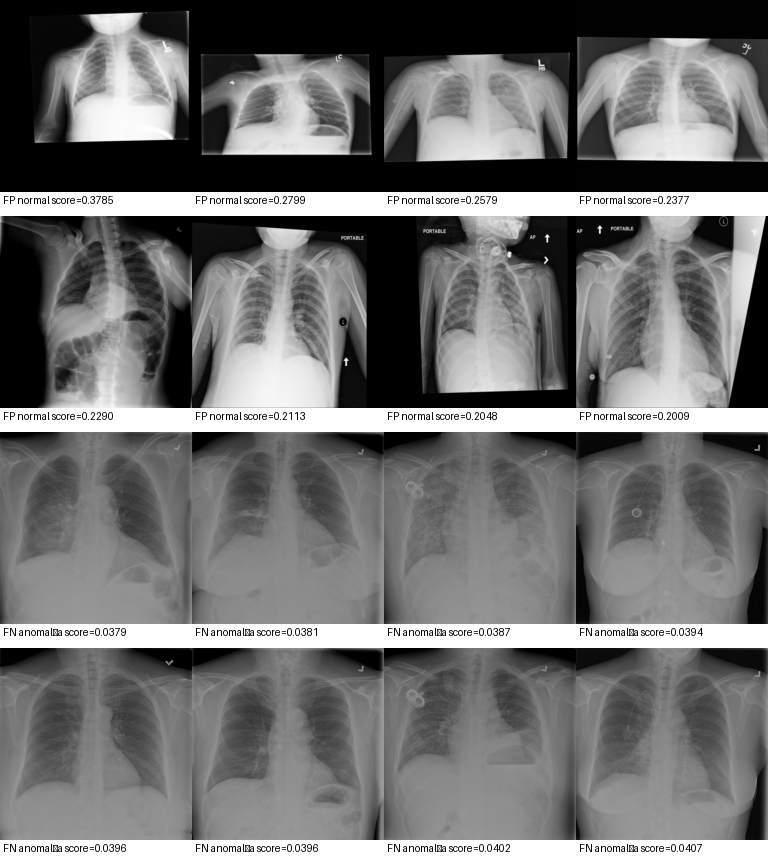
\includegraphics[width=0.92\linewidth]{errores.png}
  \caption{Falsos positivos y falsos negativos extremos de GANomaly, semilla
  42. Las miniaturas se emplean únicamente para análisis metodológico.}
\end{figure}


\section{Conclusiones}

La propuesta se ha convertido en un estudio completo: dataset auditado, tres
modelos generativos, una referencia supervisada, protocolos sin fuga, controles
simples y análisis de errores. La contribución defendible no es afirmar que un
autoencoder diagnostica patologías, sino medir bajo qué condiciones la hipótesis
de reconstrucción separa normalidad y no normalidad.

GANomaly es el mejor modelo no supervisado: supera AE y VAE en las tres semillas y
alcanza AUROC $0{,}5636\pm0{,}0150$. AE y VAE no son detectores útiles en esta
configuración, pues quedan consistentemente por debajo de 0,5 aunque reconstruyen
bien las normales. Sin embargo, el control de gradiente obtiene 0,5981 y
evidencia que variaciones simples de textura o adquisición explican una parte
importante de la separación. No se sostiene que GANomaly haya aprendido una
señal clínica robusta ni que esté preparado para uso asistencial.

El resultado es útil y defendible: demuestra experimentalmente los límites de
la hipótesis de reconstrucción, cuantifica el beneficio y coste del entrenamiento
adversarial, y detecta un atajo que quedaría oculto reportando solo AUPRC. La
conclusión negativa respecto a utilidad clínica evita una afirmación
injustificada.

La mejora mínima supervisada alcanza AUROC $0{,}8538\pm0{,}0070$ y exactitud
balanceada $0{,}7717\pm0{,}0136$. Es el resultado práctico principal del trabajo:
una arquitectura pequeña y explicable, sin ensamble ni búsqueda de algoritmos.
Su límite debe quedar explícito: aprende las etiquetas disponibles y no resuelve
la detección abierta de patologías desconocidas.

Como trabajo futuro se priorizan una ablación a 128$\times$128, validación
externa por pacientes y comparación con representaciones preentrenadas o
autoencoders enmascarados \cite{he2022mae,georgescu2023masked}. Solo después
tendría sentido estudiar localización o despliegue.


\printbibliography[title={Bibliografía}]
\end{document}
